\section*{DATA}\label{data}
The data used in this study is described in
Tab.\ref{fig:data_description}.
\begin{figure}[H]
\begin{center}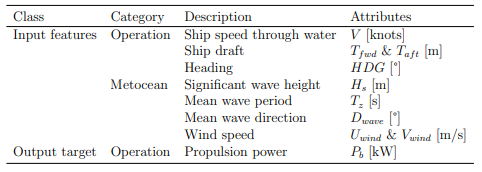
\includegraphics[width = 0.95\textwidth]{figures/data_description.png}\end{center}
\vspace{-0.7cm}
\caption{Spring-mass-damper system}
\label{fig:data_description}
\end{figure}
\subsection*{Exploratory data analysis}\label{exploratory-data-analysis}
The ship speed $V$, ship draughts $T_{aft}$ and $T_{fwd}$ were all
negative in the raw data file. This was imidiatelly corrected, to be
more in line with what would be expected from a more general sign
convention. The data seems to have been collected in time cronological
order, giving a time series of data. For a time series, measurements
close to each other in time have a high correlation, as they are
experiencing similar envinronmental conditions etc. This is confirmed by
looking at the autocorrelation plot in
Fig.\ref{fig:power_autocorrelation}. Dead reckoning (using ship
speed and heading) has been used to atempt to describe motion of the
ship as seen in Fig.\ref{fig:dead_reckoning}. The positions are
given in an unknown logintude and latitude scale, as the time step
between measurements is unknown. The speed of the ship is also indicated
as a color gradient in this figure.
\begin{verbatim}
Power          V  T_fwd  T_aft         HDG        Hs        Tz  \
0  4096.859211  23.359333  10.25   10.2  225.120423  0.336355  4.113880
1  4062.904838  23.351923  10.25   10.2  225.121609  0.334025  4.107303
2  4105.640943  23.304333  10.25   10.2  213.803859  0.331768  4.100033
3  4156.401020  23.293167  10.25   10.2  225.124531  0.328743  4.084423
4  4147.498244  23.287000  10.25   10.2  225.125682  0.326883  4.072262
D_wave    U_wind    V_wind
0  58.287071 -0.251960  0.598855
1  61.219389 -0.205543  0.537524
2  64.378446 -0.167395  0.480271
3  69.095584 -0.153352  0.410798
4  73.970302 -0.125637  0.360612
\end{verbatim}
\begin{verbatim}
Power            V        T_fwd        T_aft          HDG  \
count  8631.000000  8631.000000  8631.000000  8631.000000  8631.000000
mean   3188.935287    24.278879    11.182685    11.093998   254.571157
std    1332.289539     1.001131     0.715500     0.701950    70.481649
min    1000.000000    22.436267    10.250000    10.160000     0.000000
25%    1815.723938    23.454343    10.700000    10.600000   245.028127
50%    3173.939254    24.132437    11.000000    10.800000   270.018724
75%    4385.159249    24.897164    11.700000    11.600000   292.405334
max    5974.050320    27.955649    12.400000    12.200000   347.212496
Hs           Tz       D_wave       U_wind       V_wind
count  8631.000000  8631.000000  8631.000000  8631.000000  8631.000000
mean      1.666358     7.462152   204.735041     2.035780     0.747150
std       0.813212     1.955307    80.514470     4.931660     4.261370
min       0.158431     2.233657     2.680181   -11.236499   -14.531855
25%       1.153389     6.396379   169.396098    -0.985087    -2.065295
50%       1.540236     7.497403   205.961881     2.740314     0.088762
75%       2.160576     8.980331   268.427660     5.574664     3.568319
max       4.330742    11.513423   358.097469    13.623467    12.415640
\end{verbatim}
\begin{verbatim}
Power     float64
V         float64
T_fwd     float64
T_aft     float64
HDG       float64
Hs        float64
Tz        float64
D_wave    float64
U_wind    float64
V_wind    float64
dtype: object
\end{verbatim}
\begin{figure}[H]
\begin{center}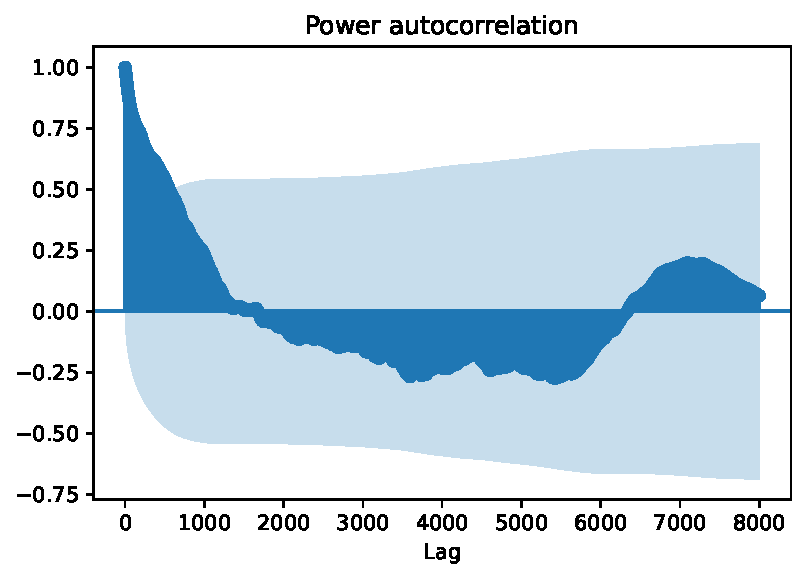
\includegraphics[width = 0.95\textwidth]{figures/power_autocorrelation.pdf}\end{center}
\vspace{-0.7cm}
\caption{Autocorrelation plot of the Power data}
\label{fig:power_autocorrelation}
\end{figure}
\begin{figure}[H]
\begin{center}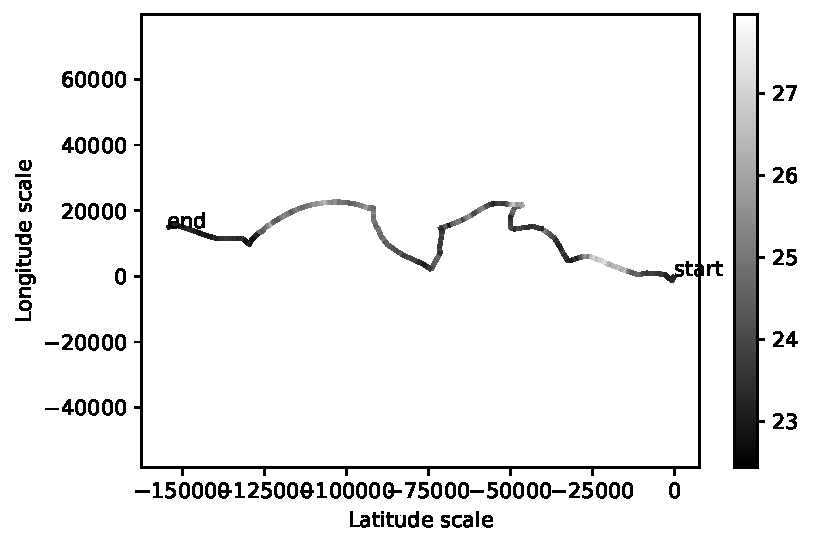
\includegraphics[width = 0.95\textwidth]{figures/dead_reckoning.pdf}\end{center}
\vspace{-0.7cm}
\caption{Dead reckoning of the position of the ship}
\label{fig:dead_reckoning}
\end{figure}
Fig.\ref{fig:heat_map_raw_data} shows a heat map of the absolute
linear correlation coefficient between all of the features in the raw
data. It can be seen that $T_{aft}$ and $T_{fwd}$ have the highest
correlation with the $Power$. It can also be seen that the correlation
between $T_{aft}$ and $T_{fwd}$ is also very high (approximately 1)
implying a very high multicollinearity which is generally something that
should be avoided in regression problems. These two features are instead
replaced with the two features: mean draught $T$ and $trim$. The
correspondig heat map with the new features is shown in
Fig.\ref{fig:heat_map_data}. The mean draught $T$ now seems to
be a very important feature in this regression as it has the highest
linear correlation with the $Power$. This can also be seen in
Fig.\ref{fig:power_draught}, where the $Power$ has been
plotted together with the corresponding negative draught.
\begin{figure}[H]
\begin{center}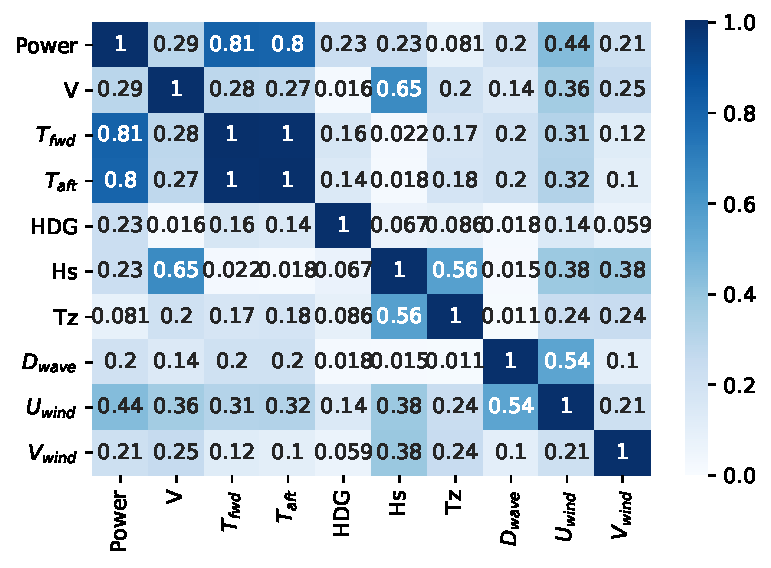
\includegraphics[width = 0.95\textwidth]{figures/heat_map_raw_data.pdf}\end{center}
\vspace{-0.7cm}
\caption{Heat map showing absolute value of correlation coefficient between features in raw data}
\label{fig:heat_map_raw_data}
\end{figure}
\begin{figure}[H]
\begin{center}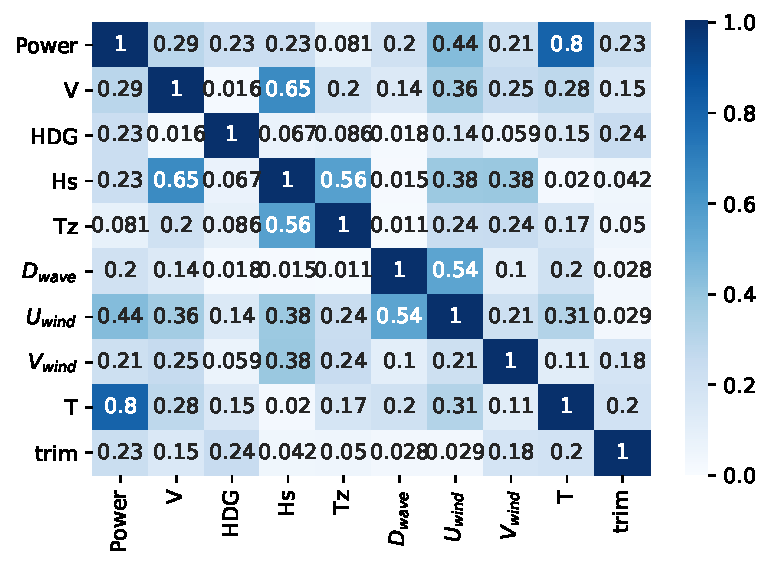
\includegraphics[width = 0.95\textwidth]{figures/heat_map_data.pdf}\end{center}
\vspace{-0.7cm}
\caption{Heat map showing absolute value of correlation coefficient between features in transformed data}
\label{fig:heat_map_data}
\end{figure}
\begin{figure}[H]
\begin{center}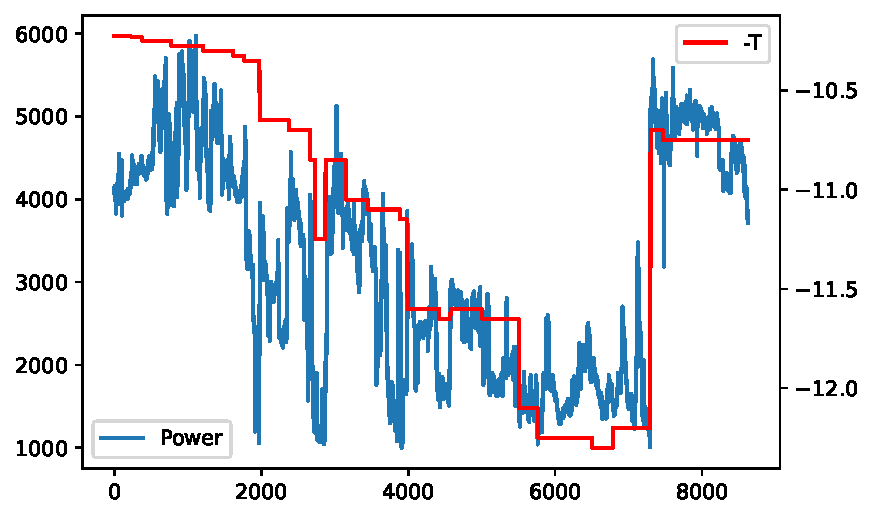
\includegraphics[width = 0.95\textwidth]{figures/power_draught.pdf}\end{center}
\vspace{-0.7cm}
\caption{The power is highly correlated with the draught}
\label{fig:power_draught}
\end{figure}
\subsection*{Extend data}\label{extend-data}
The data has also been extended by adding some additional features,
describing the wind speed and wave direction in a ship fixed coordinate
system:$u_{wind}$, $v_{wind}$, $wave_{direction}$. The new
features have very low linear correlation with $Power$ as seen in
Fig.\ref{fig:heat_map_extended_data}. They are however kept in
the data, to let the regression model decide if they are useable or not.
\begin{figure}[H]
\begin{center}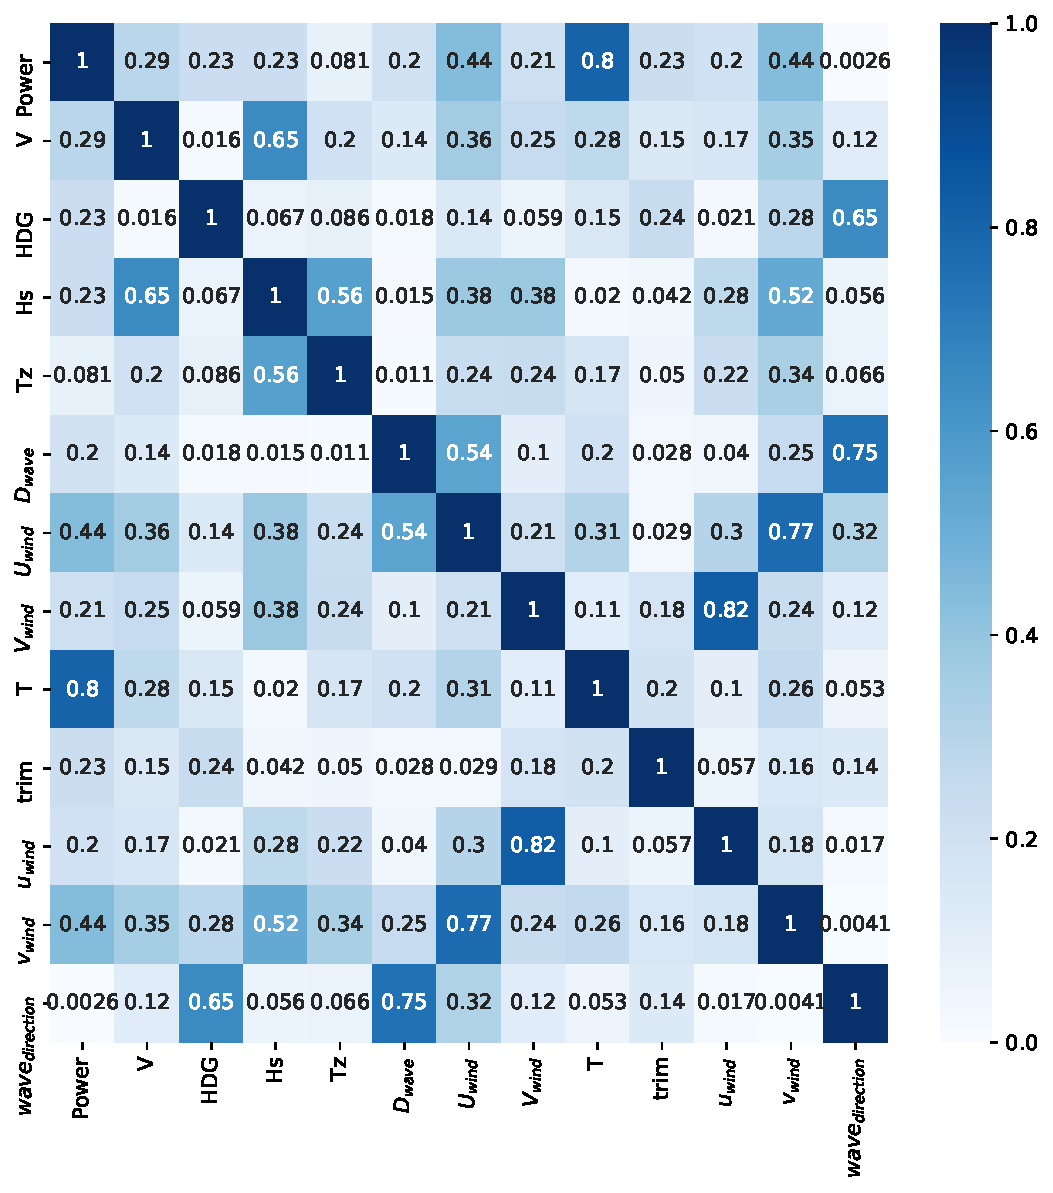
\includegraphics[width = 0.95\textwidth]{figures/output_25_0.pdf}\end{center}
\vspace{-0.7cm}
\caption{}
\label{fig:}
\end{figure}
